% chapter4.tex
% LED Chapter (Muon?)
As described in Chapter \ref{chap:muon}, the four extra modules added in 2010 covering the gap of the \mvs{} are equipped with LEDs. M7 and M8 have three LEDs: one at the center and the other two symmetrically at 0.45\,m distance from the end. M15 and M16 both have one LED installed at the center. The LEDs send out pulses every eight hours. The LED data are used to perform a stability control of the \mvs{}. They are clearly defined in light emission, position and time compared to muon induced events, therefore the LED events are a good probe to estimate the long term stability of these four modules.
\section{Data selection}
For the following analyses, data of muon-veto Run70 to Run138 are used to analyse the ageing effect of the veto system. This corresponds to a date from 24.08.2010 to 28.03.2017. When converting the raw data to ROOT-format, the events induced by LED firing are flagged. Therefore, they are easily separated from other events.
The LEDs fire three times every day. Each LED fires 60 pulses in one minute and they fire one after another, which also allows a separation of signals from different LEDs in M7 and M8.

\section{HV stability}
Since the HV information is not contained in the \textit{KData} files and the HV settings are only seldom changed over the time period, the HVs are first separately investigated. For M8, M15 and M16, the HVs are not changed from year 2010 to 2017.

\begin{figure}[htb!]
  \centering
  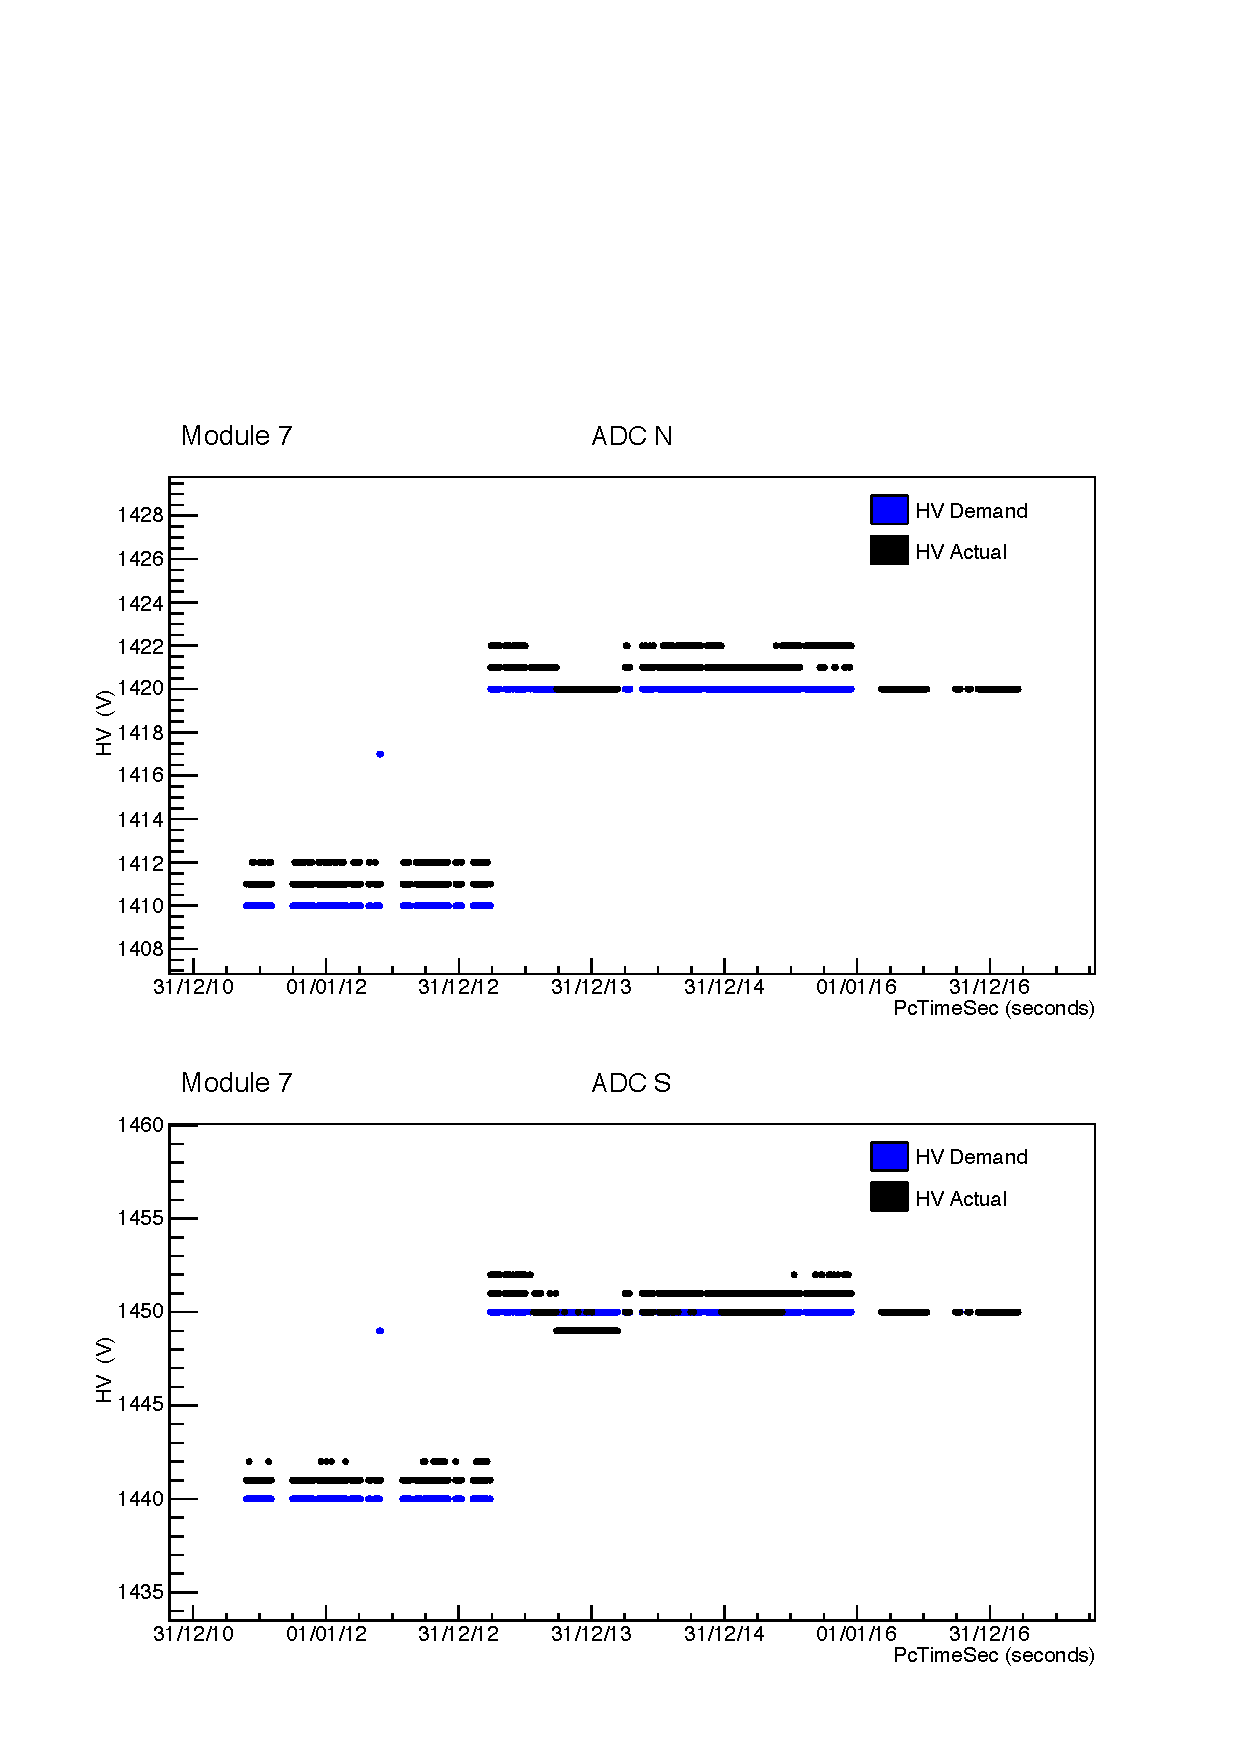
\includegraphics[width=0.8\textwidth{}]{./fig/HVPlot_M7.pdf}
  \caption{HV applied on M7 from year 2010 to 2017. The HV applied on the module is negative and the plot shows the absolute value of the HV. The blue points are the set value of the HV and the black points are the actual measured HV. In March 2013, the set HV was increased from -1410\,V to -1420\,V on the ADC N and from -1440\,V to -1450\,V on the ADC S.}
  \label{fig:HV_7}
\end{figure}

The behaviour of the HV applied on M7 is plotted in fig.\,\ref{fig:HV_7}. The plot shows the absolute value of the HV, as the HV applied on the module is actually negative. For northern PMT group, the was is increased from -1410\,V to -1420\,V in March 2013. For southern PMT group, the HV was increased from -1440\,V to -1450\,V. As seen in the figure, the measured HV values fluctuate by $\pm$3\,V from the set value.\\
For other three extra modules, the measured HV values have a fluctuation of $\pm$5\,V, which is also in the region of statistical uncertainty. The HVs are thus determined to be stable during the time period of seven years.

\section{Data Analysis}
\label{sec:led-ana}
The LEDs are fixed on the modules, so the energy spectrum is not smeared by the position dependent light readout. Also, the LEDs are supposed to have constant light output over a short time. Thus the obtained ADC spectrum can be fitted with a gaussian function to get the average ADC values of several series.
To increase the statistical power of a single point, events of nine shot series (three days) are combined to perform a gaussian fit. An example of such fit is illustrated in fig.\ref{fig:gaussian-fit}.

\begin{figure}[htb!]
  \centering
  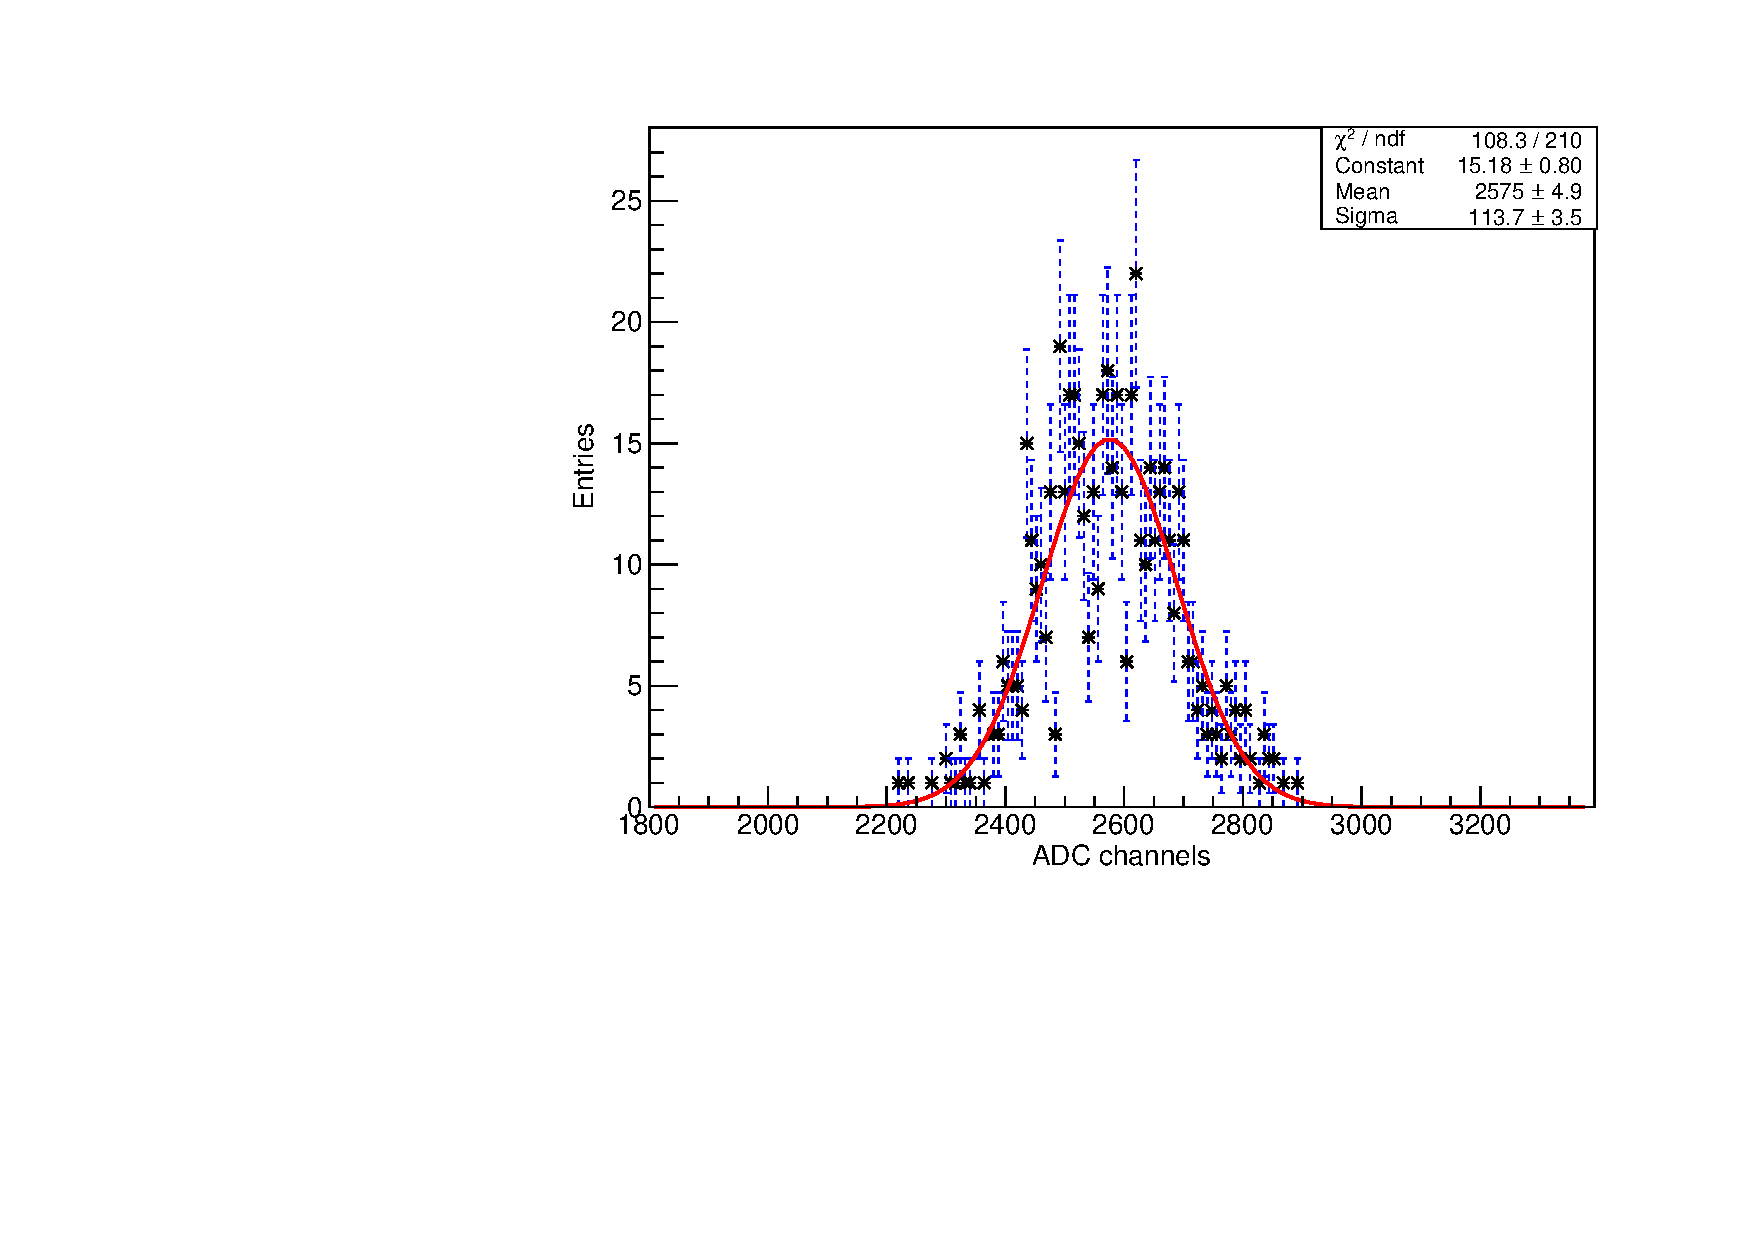
\includegraphics[width=0.8\textwidth{}]{./fig/gaussianM8.pdf}
  \caption{Example of a gaussian fit to nine LED fire series in Module 8, north PMT group. The spectrum is fitted with a log likelihood method in ROOT.}
  \label{fig:gaussian-fit}
\end{figure}

The mean ADC values obtained from each gaussian fit are plotted over time. A change of these values over time could be due to various effects, e.g.\ a decrease of the LED light output, ageing of scintillator modules, problem of the PMTs or readout electronics. To identify the contribution of different factors, the values are plotted separately for two PMT groups and three LEDs (for M7 and M8). Linear regressions are made for each data set, see fig.\ref{fig:M8LED}. The lines with different colour represent the data from different LEDs. In the following, the result is described in detail for module 8.

\begin{figure}[htbp]
  \centering
  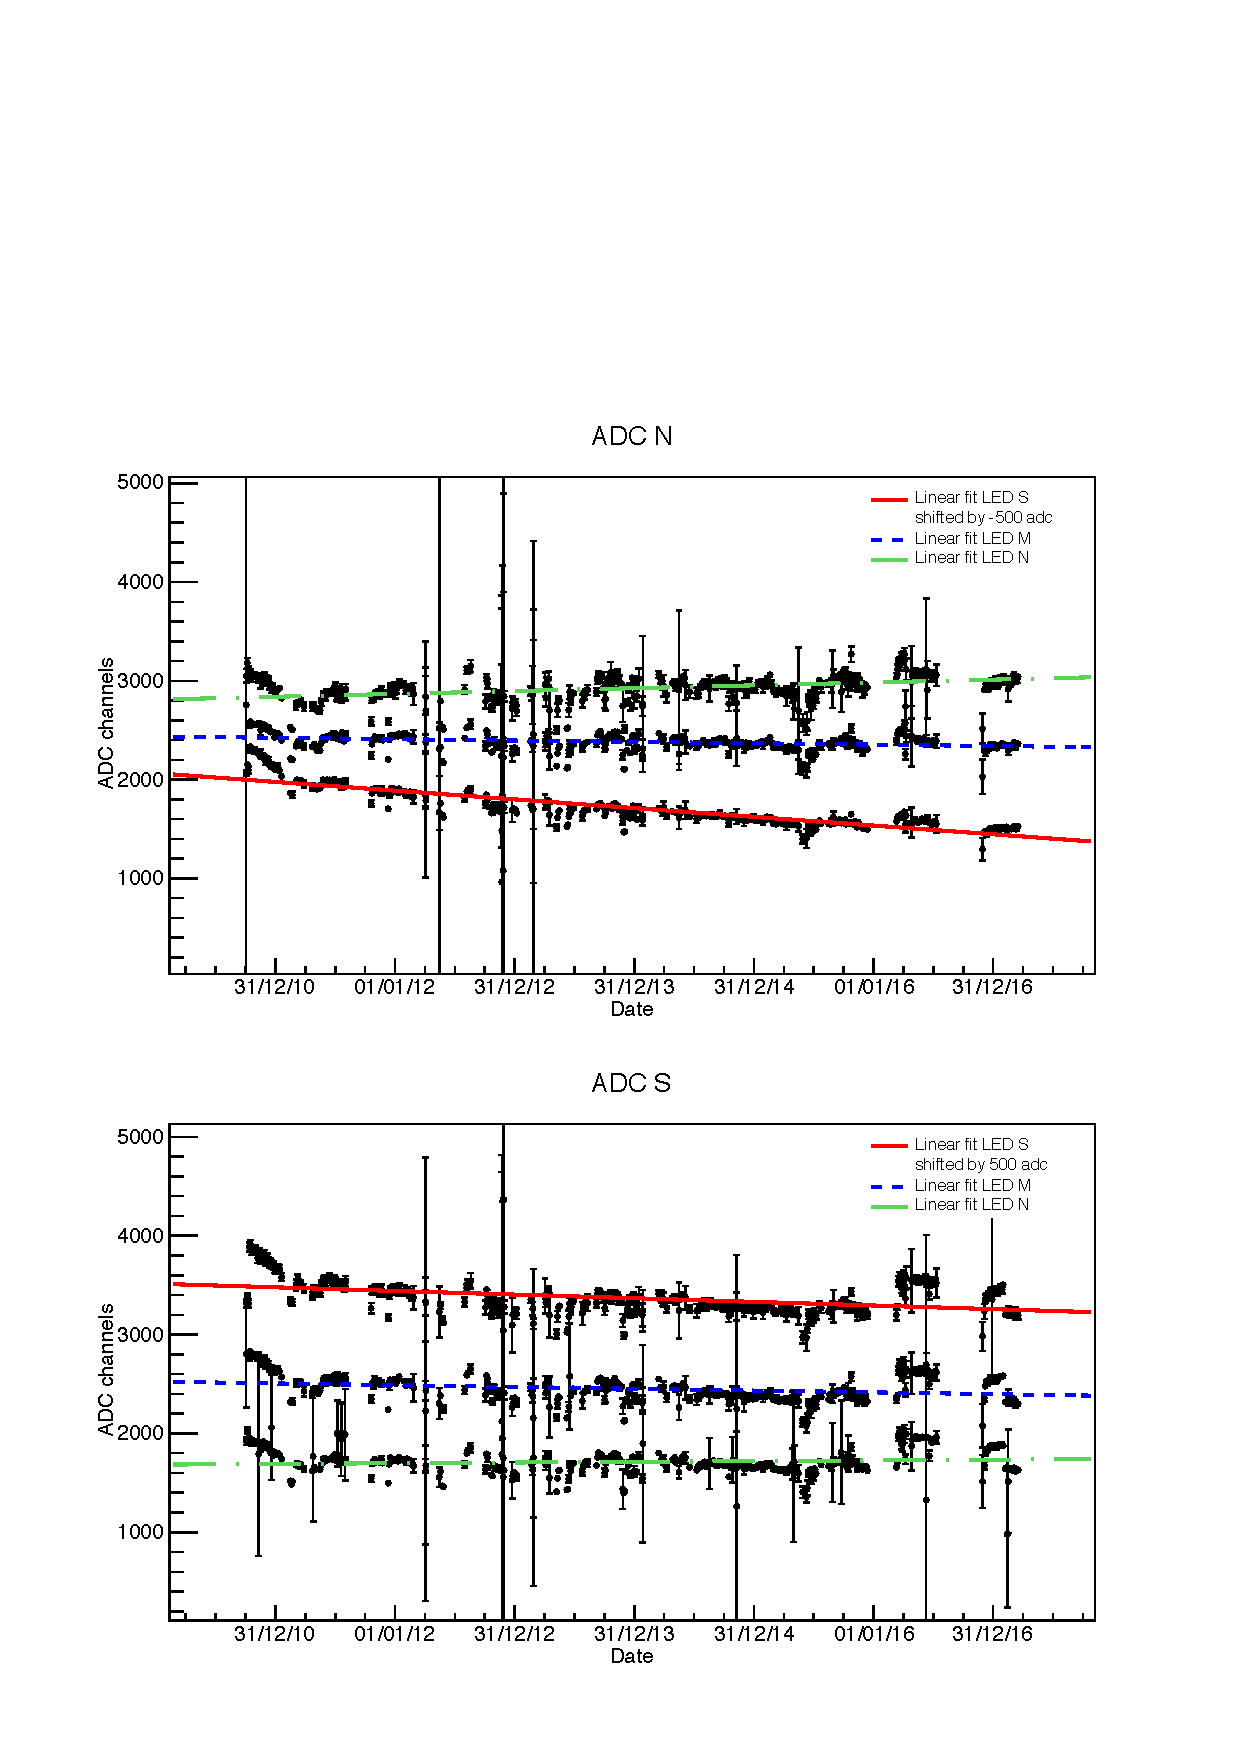
\includegraphics[width=\textwidth{}]{./fig/M8LED.pdf}
  \caption{\textbf{ADC mean values of LED signals over time in Module 8.}} The energy deposit of LED signals in ADC channels from Run70 to Run138 are plotted separately for 2 PMT groups (north in upper chart, south in lower chart). The trend of ADC values of different LEDs over time are approximated by linear fits: the green line (LED north), the blue line (LED middle), and the red line (LED south). For clarity when displaying here, the signals of the south LED are decreased by 500 channels in upper chart and increased by 500 in lower chart.
  \label{fig:M8LED}
\end{figure}

As can be seen in the figure, the mean ADC values of the two off-center LEDs differ about 500 to 1000 channels from the far end to the near end. Since M7 and M8 are only half the length of other top modules, such position dependent effects are expected to be even more remarkable in other modules.

\begin{table}[hb]
  \centering
  \caption{Slopes of the linear regressions of 3 LEDs in M8. The first uncertainty is the statistical uncertainty from the linear fit, the second is the estimated systematic uncertainty. }
  \label{tab:led}
  \begin{tabular}{c c c c}
  \toprule
        & \multicolumn{3}{c}{slope in channels/month} \\
        & LED S   & LED M  & LED N \\
  \midrule
  ADC N & $-7.26\pm0.05\pm4.32$ & $-1.13\pm0.05\pm1.06$ & $+2.37\pm0.07\pm3.12$  \\
  ADC S & $-3.02\pm0.07\pm5.50$ & $-1.49\pm0.06\pm2.92$ & $+0.59\pm0.05\pm2.74$  \\
  \bottomrule
  \end{tabular}

\end{table}

In fig.\ref{fig:M8LED}, the error bar of a single data point is the statistical uncertainty given by the gaussian fit. Since most LED events in one fire series have good gaussian form, the statistical uncertainty is mostly much smaller than the total uncertainty. Several other effects lead to the fluctuation of the ADC value, for example, the switch-on effect of electronics after a long pause. Consequently, the systematic uncertainty can only be approximated. The result of the linear fits are listed in Tab.\ref{tab:led} with uncertainty. The systematic uncertainty of the slope is estimated by fitting the first half, the middle half, and the last half of the total time period and taking the difference of the maximum and minimum slopes. \\
For example, the slope of LED S measured in the northern PMT group of M8 is estimated to be $k_{1}=-12.39\pm0.15$ channels/month for the first half (2010-2013), $k_{2}=-5.38\pm0.12$ channels/month for the middle half (2010-2013) and (2012-2015) and $k_{3}=-3.75\pm0.32$ channels/month for the last half (2014-2017). The systematic uncertainty is thus given by the half the difference between $k_{1}$ and $k_{3}$: $\Delta k_{\mathrm{sys}}=\SI{4.32}{channels/month}$.

\subsection{Discussion of the results}

Various effects could lead to the decrease or even increase of the mean ADC value of LED events. First, the transparency of plastic scintillator decreases over time. Assuming that such ageing effect is homogeneous in one module, the loss of light output depends on the distance from the event position to the PMT group. This leads to roughly the same decrease for events that have same track length to the PMT group, e.g. LED N to ADC S and LED S to ADC N. Second, the PMTs as well as the junction of scintillator module and PMT group have aged individually, which leads to different variation of ADC values at two ends of a module. Last, the light output of an LED may vary over time and thus leads to the simultaneous change of measured values in two PMT groups.

The slopes of middle LED in two ends of M8 are about the same, implying that the two PMT groups of M8 have aged similarly. Therefore the ageing effect of the plastic scintillator can be estimated by subtracting the slope of the same LED at the near end from the one at the far end. \\
For LED S, this value is $\Delta{}_{\mathrm{LED\,S}}=\SI{-4.2}{channels\per month}$ and for LED N $\Delta{}_{\mathrm{LED \,N}}=\SI{-1.8}{channels\per month}$. The values vary much from each other but still lie in the region of estimated uncertainty. This implies that the systematic uncertainty is indeed large, as these two values are expected to be the same for a homogeneous ageing of the scintillator.

Furthermore the decrease is noticeably more rapid at earlier stage (about 2010-2011) and becomes flat later. The reason can be that the transparency loss of scintillator is not linear over time. The assumption of a linear trend is thus only an approximation.
Averaging over time, the decrease due to ageing of plastic scintillator is estimated to correspond to  $\approx \SI{3}{channels\per month}$. During the total period of experiment (about $\SI{90}{months}$), the change of ADC values caused by scintillator ageing is about $\SI{250}{channels}$ for M8. Given the start values of $\approx$2500\,ch for LED pulses, this corresponds to roughly 10\% loss in light output for an event at a distance about 1.65\,m from a PMT group.

The same procedure is applied on other three modules M7,M15 and M16 and shows similar results. Since other modules are longer then the four modules, the decrease of ADC values are expected to be more significant. This is in fact the case, see table \ref{tab:mpv}. Consequently, the detection efficiency of a individual module reduces, especially for events to be measured in the far PMT group, as the transportation length of light is longer.

\subsection{Conclusion}

To conclude, the analysis of LED events shows that the gain of PMT groups has decreased. Although the change is negligible for a short period, it becomes significant accumulating over the long time period of seven years.

In this chapter, LED events are used to investigate the ageing effect of the muon-veto scintillator modules. This method has the advantage that the selected events are pure LED events, unlike the selection of muon events which always contains certain backgrounds. In addition, the measured energy spectrum of LED events is gaussian distributed and the mean ADC values can be easily determined. \\
Moreover, every measured LED event can be associated to a certain LED, or correspondingly a certain position. As described above, this allows to separate the effects of different sources on the ageing of a module. For example, the difference of mean ADC values of LED N in two PMT groups gives a measure of the transparency loss of the scintillator. Though the position of muon events can also be reconstructed by the difference of two TDC values, the ageing effects of different sources cannot be reliably separated due to the low statistics and the wide energy spectrum of muon-induced events.

On the other hand, this method using LED events also has its limitations. First of all, the result obtained here only shows qualitatively that the modules have aged. It gives little information on the actual effect on the change of the muon detection efficiency, which is essential for the experiment. Also, as mentioned before, only four extra modules are equipped with LEDs. The other modules cannot be investigated using this method. To achieve that, muon induced events are analysed in the next chapter.





%discussion, pro and cons of LED vs muon events ...
%relation to muon efficiency
